% Définition d'une commande :
% #1 = options TikZ (couleur, etc.)
% #2 = centre (ex: (2,3))
% #3 = échelle (taille)
\newcommand{\patatoide}[3][]{%
\begin{scope}[shift={#2}, scale=#3]
\draw[#1]
plot[smooth cycle, tension=1]
coordinates {
(0,0)
(1,0.3)
(1.3,1.2)
(0.3,1.8)
(-0.8,1.2)
(-1,0.2)
};

\node at (0,-0.25) {$\Gamma_{s, f}^1$};
\node at (0.4,1) {$\Omega_{s}^1$};

\draw[<->, red , decorate, decoration={zigzag, amplitude=2pt}]
    (1.2,0.5) -- (5,1);
    
\draw[<->, red , decorate, decoration={zigzag, amplitude=2pt}]
    (-1, 1) -- (-2.5,2);
    
\draw[<->, red , decorate, decoration={zigzag, amplitude=2pt}]
    (0.5, 1.8) -- (2.1,2.7);
\end{scope}
}

\newcommand{\patatoideThin}[3][]{%
\begin{scope}[shift={#2}, scale=#3]
\draw[#1]
plot[smooth cycle, tension=1]
coordinates {
(0,0)
(0.7,0.3)
(1,1.2)
(0.1,1.8)
(-0.6,1.2)
(-0.8,0.2)
};
\node at (1.3,1.6) {$\Gamma_{s, f}^2$};
\node at (0.4,1) {$\Omega_{s}^2$};
\draw[<->, red , decorate, decoration={zigzag, amplitude=2pt}]
    (1, -0.8) -- (0,0);
\end{scope}
}
\newcommand{\patatoideInv}[3][]{%
\begin{scope}[shift={#2}, scale=#3]
\draw[#1]
plot[smooth cycle, tension=1]
coordinates {
(0,0)
(-1,-0.3)
(-1.3,-1.2)
(-0.3,-1.8)
(0.8,-1.2)
(1,-0.2)
};
\node at (0,-1.85) {$\Gamma_{f}$};
\node at (-0.1,-1.4) {$\Omega_{f}$};
\draw[<->, red , decorate, decoration={zigzag, amplitude=2pt}]
    (-0.2, -1.8) -- (0.43,-1.6);
\end{scope}
}
\newcommand{\patatoideThinInv}[3][]{%
\begin{scope}[shift={#2}, scale=#3]
\draw[#1]
plot[smooth cycle, tension=1]
coordinates {
(0,0)
(-0.7,-0.3)
(-1,-1.2)
(-0.1,-1.8)
(0.6,-1.2)
(0.8,-0.2)
};
\node at (0,0.2) {$\Gamma_{s, f}^3$};
\node at (0,-1) {$\Omega^3_{s}$};

\draw[<->, red , decorate, decoration={zigzag, amplitude=2pt}]
    (0.7, -1) -- (1.2,-1.5);
\draw[<->, red , decorate, decoration={zigzag, amplitude=2pt}]
    (0.8, -0.2) -- (2.8,0);
\end{scope}
}




\begin{minipage}{0.7\textwidth}

    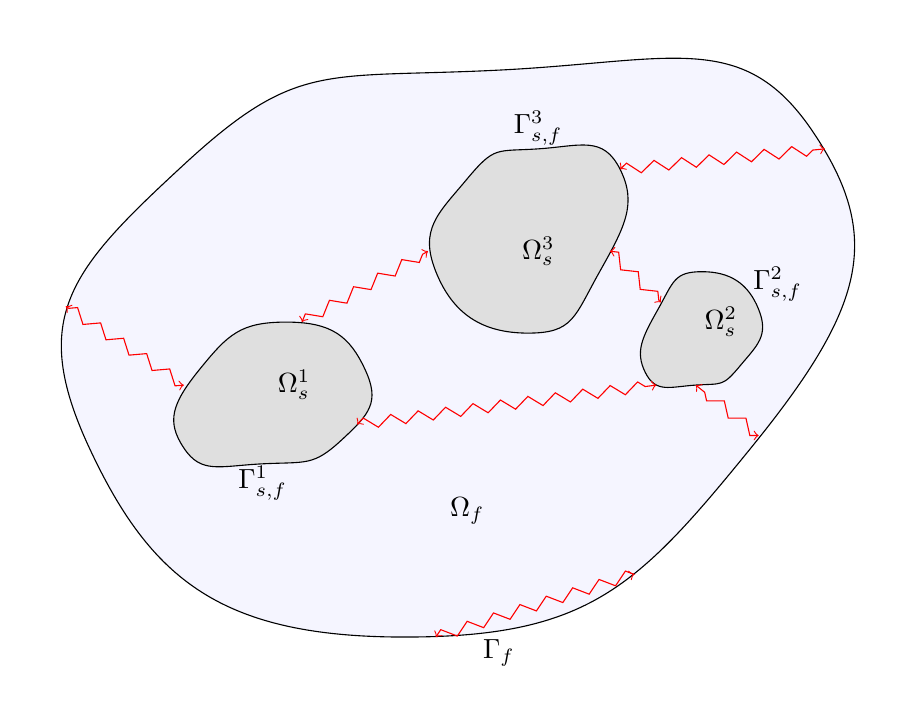
\begin{tikzpicture}
        \patatoideInv[fill=blue!4, draw=black]{(0,0)}{4}
        \patatoideThin[fill=gray!25, draw=black]{(2.5,-4)}{0.8}
        \patatoideThinInv[fill=gray!25, draw=black]{(0.5,-1)}{1.3}
        \patatoide[fill=gray!25, draw=black]{(-3,-5)}{1}
    \end{tikzpicture}


    \caption{Schéma typique d’un problème de couplage conduction-rayonnement en milieu transparent}
    \label{fig:domaine}
\end{minipage}